\documentclass[12pt,letterpaper]{article}
\usepackage{graphicx,textcomp}
\usepackage{natbib}
\usepackage{setspace}
\usepackage{fullpage}
\usepackage{color}
\usepackage[reqno]{amsmath}
\usepackage{amsthm}
\usepackage{fancyvrb}
\usepackage{amssymb,enumerate}
\usepackage[all]{xy}
\usepackage{endnotes}
\usepackage{lscape}
\newtheorem{com}{Comment}
\usepackage{float}
\usepackage{hyperref}
\newtheorem{lem} {Lemma}
\newtheorem{prop}{Proposition}
\newtheorem{thm}{Theorem}
\newtheorem{defn}{Definition}
\newtheorem{cor}{Corollary}
\newtheorem{obs}{Observation}
\usepackage[compact]{titlesec}
\usepackage{dcolumn}
\usepackage{tikz}
\usetikzlibrary{arrows}
\usepackage{multirow}
\usepackage{xcolor}
\newcolumntype{.}{D{.}{.}{-1}}
\newcolumntype{d}[1]{D{.}{.}{#1}}
\definecolor{light-gray}{gray}{0.65}
\usepackage{url}
\usepackage{listings}
\usepackage{color}

\definecolor{codegreen}{rgb}{0,0.6,0}
\definecolor{codegray}{rgb}{0.5,0.5,0.5}
\definecolor{codepurple}{rgb}{0.58,0,0.82}
\definecolor{backcolour}{rgb}{0.95,0.95,0.92}

\lstdefinestyle{mystyle}{
	backgroundcolor=\color{backcolour},   
	commentstyle=\color{codegreen},
	keywordstyle=\color{magenta},
	numberstyle=\tiny\color{codegray},
	stringstyle=\color{codepurple},
	basicstyle=\footnotesize,
	breakatwhitespace=false,         
	breaklines=true,                 
	captionpos=b,                    
	keepspaces=true,                 
	numbers=left,                    
	numbersep=5pt,                  
	showspaces=false,                
	showstringspaces=false,
	showtabs=false,                  
	tabsize=2
}
\lstset{style=mystyle}
\newcommand{\Sref}[1]{Section~\ref{#1}}
\newtheorem{hyp}{Hypothesis}

\title{Problem Set 3}
\date{Due: March 24, 2024}
\author{Applied Stats II}


\begin{document}
	\maketitle
	\section*{Instructions}
	\begin{itemize}
	\item Please show your work! You may lose points by simply writing in the answer. If the problem requires you to execute commands in \texttt{R}, please include the code you used to get your answers. Please also include the \texttt{.R} file that contains your code. If you are not sure if work needs to be shown for a particular problem, please ask.
\item Your homework should be submitted electronically on GitHub in \texttt{.pdf} form.
\item This problem set is due before 23:59 on Sunday March 24, 2024. No late assignments will be accepted.
	\end{itemize}

	\vspace{.25cm}
\section*{Question 1}
\vspace{.25cm}
\noindent We are interested in how governments' management of public resources impacts economic prosperity. Our data come from \href{https://www.researchgate.net/profile/Adam_Przeworski/publication/240357392_Classifying_Political_Regimes/links/0deec532194849aefa000000/Classifying-Political-Regimes.pdf}{Alvarez, Cheibub, Limongi, and Przeworski (1996)} and is labelled \texttt{gdpChange.csv} on GitHub. The dataset covers 135 countries observed between 1950 or the year of independence or the first year forwhich data on economic growth are available ("entry year"), and 1990 or the last year for which data on economic growth are available ("exit year"). The unit of analysis is a particular country during a particular year, for a total $>$ 3,500 observations. 

\begin{itemize}
	\item
	Response variable: 
	\begin{itemize}
		\item \texttt{GDPWdiff}: Difference in GDP between year $t$ and $t-1$. Possible categories include: "positive", "negative", or "no change"
	\end{itemize}
	\item
	Explanatory variables: 
	\begin{itemize}
		\item
		\texttt{REG}: 1=Democracy; 0=Non-Democracy
		\item
		\texttt{OIL}: 1=if the average ratio of fuel exports to total exports in 1984-86 exceeded 50\%; 0= otherwise
	\end{itemize}
	
\end{itemize}
\newpage
\noindent Please answer the following questions:

\begin{enumerate}
	\item Construct and interpret an unordered multinomial logit with \texttt{GDPWdiff} as the output and "no change" as the reference category, including the estimated cutoff points and coefficients.
\subsection*{Answer:}

\begin{lstlisting}[language=R]
	# Change GDPWdiff from numeric to categorical, and then factor with reference.
	
	gdp_data$GDPWdiff <- ifelse(gdp_data$GDPWdiff == 0, "no change", 
	ifelse(gdp_data$GDPWdiff > 0, "positive", "negative"))
	
	gdp_data$GDPWdiff <- factor(gdp_data$GDPWdiff, ordered = FALSE)
	
	gdp_data$GDPWdiff <- relevel(gdp_data$GDPWdiff, ref = "no change")
	
	model <- multinom(GDPWdiff ~ REG + OIL, data = gdp_data)
\end{lstlisting}

\begin{table}[!htbp] \centering 
	\caption{the estimated coefficients of the unordered multinomial logistic regression} 
	\label{} 
	\begin{tabular}{@{\extracolsep{5pt}}lcc} 
		\\[-1.8ex]\hline 
		\hline \\[-1.8ex] 
		& \multicolumn{2}{c}{\textit{Dependent variable:}} \\ 
		\cline{2-3} 
		\\[-1.8ex] & negative & positive \\ 
		\\[-1.8ex] & (1) & (2)\\ 
		\hline \\[-1.8ex] 
		REG & 1.379$^{*}$ & 1.769$^{**}$ \\ 
		& (0.769) & (0.767) \\ 
		& & \\ 
		OIL & 4.784 & 4.576 \\ 
		& (6.885) & (6.885) \\ 
		& & \\ 
		Constant & 3.805$^{***}$ & 4.534$^{***}$ \\ 
		& (0.271) & (0.269) \\ 
		& & \\ 
		\hline \\[-1.8ex] 
		Akaike Inf. Crit. & 4,690.770 & 4,690.770 \\ 
		\hline 
		\hline \\[-1.8ex] 
		\textit{Note:}  & \multicolumn{2}{r}{$^{*}$p$<$0.1; $^{**}$p$<$0.05; $^{***}$p$<$0.01} \\ 
	\end{tabular} 
\end{table} 

	The constant (or cutoff point) 3.805 is the log odds that GDPWdiff will be negative relative to the baseline category of no change when both REG and OIL are coded as zero. The constant (or cutoff point) 4.534 is the log odds that GDPWdiff will be positive relative the baseline category of no change when both REG and OIL are coded as zero.

	For a one unit increase in REG, that being when a country goes from being coded as 0 (non-democracy) to 1(democracy), there is a 1.379 unit increase in the log odds of GDPWdiff being negative vs the baseline category of no change. There is also a 1.769 unit increase in the log odds of GDPWdiff being positive vs the baseline category.
	
	For a one unit increase in OIL, that being when a county goes from being coded as one in which the ratio of fuel exports to total exports does not exceed 50\% (0), to one in which it does (1), there is a 4.784 unit increase in the log odds of GDPWdiff being negative vs the baseline category of no change. There is also a 4.576 unit increase in the log odds of GDPWdiff being positive vs the baseline category.
	
	\vspace{1cm}

\begin{table}[!htbp] \centering 
	\caption{the exponents of the coefficients (the odds) from the multinominal logistic regression model} 
	\label{} 
	\begin{tabular}{@{\extracolsep{5pt}} cccc} 
		\\[-1.8ex]\hline 
		\hline \\[-1.8ex] 
		& (Intercept) & REG & OIL \\ 
		\hline \\[-1.8ex] 
		negative & $44.942$ & $3.972$ & $119.578$ \\ 
		positive & $93.108$ & $5.865$ & $97.156$ \\ 
		\hline \\[-1.8ex] 
	\end{tabular} 
\end{table}  

44.942 represents the multiplicative change in the odds that GDPWdiff will be negative vs the baseline category of no change when both REG and OIL are coded as zero 93.108 represents the multiplicative change in the odds that GDPWdiff will be positive vs the baseline category of no change when both REG and OIL are coded as zero.

3.972 represents the multiplicative change in the odds that GDPWdiff will be negative vs the baseline category of no change when REG changes from 0 to 1. 5.856 represents the multiplicative change in the odds that GDPWdiff will be positive vs the baseline category of no change when REG changes from 0 to 1.

119.578 represents the multiplicative change in the odds that GDPWdiff will be negative vs the baseline category of no change when OIL changes from 0 to 1. 97.156 represents the multiplicative change in the odds that GDPWdiff will be positive vs the baseline category of no change when OIL changes from 0 to 1.


	\item Construct and interpret an ordered multinomial logit with \texttt{GDPWdiff} as the outcome variable, including the estimated cutoff points and coefficients.
\subsection*{Answer:}
	
\begin{lstlisting}[language=R]
	# Order the factors.
	gdp_data$GDPWdiff <- factor(gdp_data$GDPWdiff, ordered = TRUE, levels = c("negative", "no change", "positive"))
	
	model2 <- polr(GDPWdiff ~ REG + OIL, data = gdp_data)
\end{lstlisting}

\begin{table}[!htbp] \centering 
	\caption{the estimated coefficients of the ordinal multinomial logistic regression model2} 
	\label{} 
	\begin{tabular}{@{\extracolsep{5pt}}lc} 
		\\[-1.8ex]\hline 
		\hline \\[-1.8ex] 
		& \multicolumn{1}{c}{\textit{Dependent variable:}} \\ 
		\cline{2-2} 
		\\[-1.8ex] & GDPWdiff \\ 
		\hline \\[-1.8ex] 
		REG & 0.398$^{***}$ \\ 
		& (0.075) \\ 
		& \\ 
		OIL & $-$0.199$^{*}$ \\ 
		& (0.116) \\ 
		& \\ 
		\hline \\[-1.8ex] 
		Observations & 3,721 \\ 
		\hline 
		\hline \\[-1.8ex] 
		\textit{Note:}  & \multicolumn{1}{r}{$^{*}$p$<$0.1; $^{**}$p$<$0.05; $^{***}$p$<$0.01} \\ 
	\end{tabular} 
\end{table} 

\begin{table}[!htbp] \centering 
	\caption{the estimated odds ratios and their confidence intervals of the ordinal multinominal logistic regression model2.} 
	\label{} 
	\begin{tabular}{@{\extracolsep{5pt}} cccc} 
		\\[-1.8ex]\hline 
		\hline \\[-1.8ex] 
		& OR & 2.5 \% & 97.5 \% \\ 
		\hline \\[-1.8ex] 
		REG & $1.490$ & $1.286$ & $1.727$ \\ 
		OIL & $0.820$ & $0.655$ & $1.031$ \\ 
		\hline \\[-1.8ex] 
	\end{tabular} 
\end{table} 

For every one unit increase in REG there is an approximate 0.398 increase in the log odds of moving from a lower category of GDPWdiff (e.g., negative or no change) to a higher category (e.g., no change or positive), holding the other variables constant.

For every one unit increase in OIL there is an approximate 0.199 decrease in the log odds of moving from a lower category of GDPWdiff to a higher category, holding other variables constant.

\begin{table}[htbp]
	\centering
	\caption{Intercepts (cutoff points) of the ordinal multinomial regression model2}
	\begin{tabular}{lccc}
		\hline
		\hline
		& Value & Std. Error & t value \\
		\hline
		negative|no change & -0.7312 & 0.0476 & -15.3597 \\
		no change|positive & -0.7105 & 0.0475 & -14.9554 \\
		\hline
		\hline
	\end{tabular}%
	\label{tab:intercepts}%
\end{table}%

-0.7312 represents the log odds of being in the negative category of GDPWdiff relative to no change category, when both OIL and REG are at zero, it is the baseline log odds of the negative category relative to the no change category.

-0.7105 represents the log odds of being in the no change category of GDPWdiff relative to the positive category, when both OIL and REG are at zero, it is the baseline log odds of the no change category relative to positive category.

	
\end{enumerate}

\section*{Question 2} 
\vspace{.25cm}

\noindent Consider the data set \texttt{MexicoMuniData.csv}, which includes municipal-level information from Mexico. The outcome of interest is the number of times the winning PAN presidential candidate in 2006 (\texttt{PAN.visits.06}) visited a district leading up to the 2009 federal elections, which is a count. Our main predictor of interest is whether the district was highly contested, or whether it was not (the PAN or their opponents have electoral security) in the previous federal elections during 2000 (\texttt{competitive.district}), which is binary (1=close/swing district, 0="safe seat"). We also include \texttt{marginality.06} (a measure of poverty) and \texttt{PAN.governor.06} (a dummy for whether the state has a PAN-affiliated governor) as additional control variables. 

\begin{enumerate}
	\item [(a)]
	Run a Poisson regression because the outcome is a count variable. Is there evidence that PAN presidential candidates visit swing districts more? Provide a test statistic and p-value.
	
\subsection*{Answer:}

The Poisson regression can be run with the following code.

\begin{lstlisting}[language=R]
	model3 <- glm(PAN.visits.06 ~ competitive.district
	+ marginality.06 + PAN.governor.06,
	family = "poisson", data = mexico_elections)
\end{lstlisting}

\vspace{1cm}

\begin{table}[!htbp] \centering 
	\caption{the estimated coefficients of the Poisson regression} 
	\label{} 
	\begin{tabular}{@{\extracolsep{5pt}}lc} 
		\\[-1.8ex]\hline 
		\hline \\[-1.8ex] 
		& \multicolumn{1}{c}{\textit{Dependent variable:}} \\ 
		\cline{2-2} 
		\\[-1.8ex] & PAN.visits.06 \\ 
		\hline \\[-1.8ex] 
		competitive.district & $-$0.081 \\ 
		& (0.171) \\ 
		& \\ 
		marginality.06 & $-$2.080$^{***}$ \\ 
		& (0.117) \\ 
		& \\ 
		PAN.governor.06 & $-$0.312$^{*}$ \\ 
		& (0.167) \\ 
		& \\ 
		Constant & $-$3.810$^{***}$ \\ 
		& (0.222) \\ 
		& \\ 
		\hline \\[-1.8ex] 
		Observations & 2,407 \\ 
		Log Likelihood & $-$645.606 \\ 
		Akaike Inf. Crit. & 1,299.213 \\ 
		\hline 
		\hline \\[-1.8ex] 
		\textit{Note:}  & \multicolumn{1}{r}{$^{*}$p$<$0.1; $^{**}$p$<$0.05; $^{***}$p$<$0.01} \\ 
	\end{tabular} 
\end{table} 

\vspace{4cm}

\begin{table}[!htbp] \centering 
	\caption{the odds ratios and their confidence intervals for model3} 
	\label{} 
	\begin{tabular}{@{\extracolsep{5pt}} cccc} 
		\\[-1.8ex]\hline 
		\hline \\[-1.8ex] 
		& OR & 2.5 \% & 97.5 \% \\ 
		\hline \\[-1.8ex] 
		(Intercept) & $0.022$ & $0.014$ & $0.034$ \\ 
		competitive.district & $0.922$ & $0.666$ & $1.302$ \\ 
		marginality.06 & $0.125$ & $0.099$ & $0.156$ \\ 
		PAN.governor.06 & $0.732$ & $0.523$ & $1.007$ \\ 
		\hline \\[-1.8ex] 
	\end{tabular} 
\end{table} 

\vspace{1cm}

\begin{table}[ht]
	\centering
		\caption{the estimated coefficients along with their test statistics and p-values for model3} 
	\label{} 
	\begin{tabular}{rrrrr}
		\hline
		& Estimate & Std. Error & z value & Pr($>$$|$z$|$) \\ 
		\hline
		(Intercept) & -3.8102 & 0.2221 & -17.16 & 0.0000 \\ 
		competitive.district & -0.0814 & 0.1707 & -0.48 & 0.6336 \\ 
		marginality.06 & -2.0801 & 0.1173 & -17.73 & 0.0000 \\ 
		PAN.governor.06 & -0.3116 & 0.1667 & -1.87 & 0.0617 \\ 
		\hline
	\end{tabular}
\end{table}



Null Hypothesis (H0) = There is not enough evidence to support the claim that PAN presidential candidates visit swing districts more.

Alternative Hypothesis (HA) = There is sufficient evidence to support the claim that PAN presidential candidates visit swing districts more.

Given the p-value for the coefficient competitive.district is equal to 0.6336 and this is greater than the level of significance ($\alpha$ = 0.05) \textbf{we fail to reject the null hypothesis, there is not enough evidence to support the claim that PAN presidential candidates visit swing districts more.}

Given the low explanatory capability of the model in this case, it is worth trying a zero inflated Poisson model on the data to see if they are zero inflated.

\begin{figure}[tbph]
	\centering
	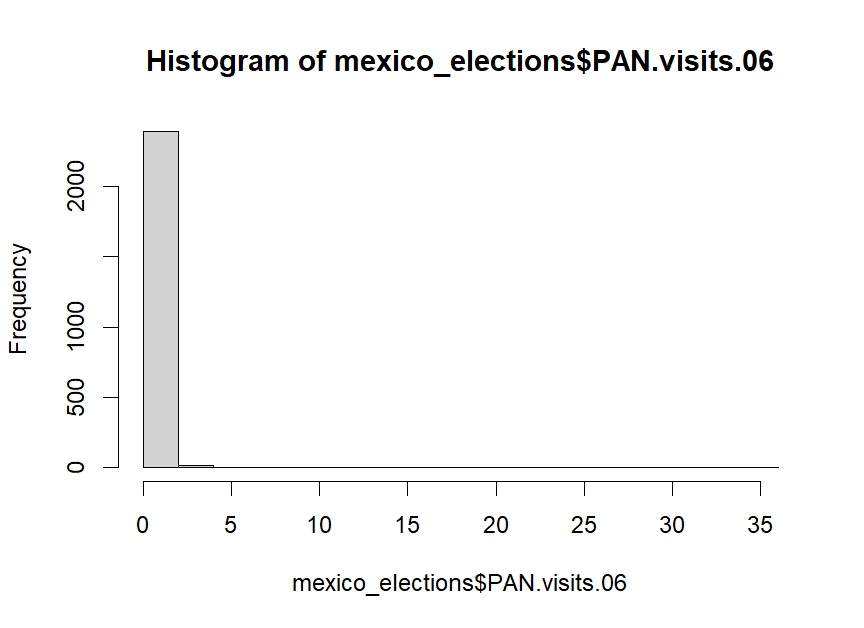
\includegraphics[width=0.8\linewidth]{../../../../../../../Documents/mehist}
	\caption{Frequency of number of PAN visits}
	\label{fig:mehist}
\end{figure}

\vspace{7cm}

This histogram of the frequency of each number of PAN visits would suggest that zeros are over represented in the data.

\begin{lstlisting}[language=R]
	library(pscl)
	zip_model3 <- zeroinfl(PAN.visits.06 ~ competitive.district
	+ marginality.06 + PAN.governor.06,
	data = mexico_elections, dist = "poisson")
	
	# Test the models.
	
	library(AER)
	dispersiontest(model3)
	AIC (model3, zip_model3)
\end{lstlisting}

After running and testing the zero inflated model is seems the model could be somewhat zero inflated but the high p-value \textbf{0.143} of the dispersion test suggests that there is not sufficient evidence to make that claim. Also looking at the coefficients and p-values of the zero inflated model it does not appear to offer more useful insights than the regular Poisson model, e.g. the coefficient p-values are similar. Refer to R file for more details.

	\item [(b)]
	Interpret the \texttt{marginality.06} and \texttt{PAN.governor.06} coefficients.
	

\subsection*{Answer:}

\textbf{marginality.06:} for every one unit increase in marginality.06 there is approximately a 2.080 decrease in the log count of PAN presidential visits, holding all other variables constant.

\textbf{PAN.governor.06:} for a one unit increase in PAN.governor.06, that being when a hypothetical district goes from not having a PAN affiliated governor to having a PAN affiliated governor, there is an approximate 0.312 decrease in the log count of PAN presidential visits, holding all other variables constant. Although considering the high p-value of the PAN.governor.06 coefficient, 0.0617 \(>\alpha=0.05\), the effect of this coefficient is not statistically significant.
	
	
	\item [(c)]
	Provide the estimated mean number of visits from the winning PAN presidential candidate for a hypothetical district that was competitive (\texttt{competitive.district}=1), had an average poverty level (\texttt{marginality.06} = 0), and a PAN governor (\texttt{PAN.governor.06}=1).
	
\subsection*{Answer:}

The following R code is used to do the calculation:
\begin{lstlisting}[language=R]
	exp(model3_cfs[1] + model3_cfs[2]*1 + model3_cfs[3]*0 + model3_cfs[4]*1)
\end{lstlisting}

It does the calculation by getting the exponent of the regression equation for the regression model3, getting the exponent works as a link function in the case of Poisson regression.

The calculation provides a result \textbf{= 0.0149} which means that the estimated mean number of visits from the winning PAN presidential candidate for a hypothetical district that was competitive, had an average poverty level, and a PAN governor was 0.0149. 

\subsection*{Bibliography:}

\begin{itemize}
	\item Zhang, Z. (no date) ‘Estimating The Optimal Cutoff Point For Logistic Regression’.
	\item Kwak, C. and Clayton-Matthews, A. (2002) ‘Multinomial Logistic Regression’, Nursing Research, 51(6), p. 404.
	\item O’Halloran, S. (no date) ‘Lecture 10: Logistical Regression II— Multinomial Data’.
	\item Mokhtar, K.I., Wan Nor Arifin, Tengku Muhammad Hanis Tengku (no date) Chapter 9 Multinomial Logistic Regression | Data Analysis in Medicine and Health using R. (Accessed: 23 March 2024).
	\item Faraway, J.J. (2016) Extending the Linear Regression Model with R, second edition.
	\item Dr. Jeffrey Ziegler's lecture material.
\end{itemize}

	
\end{enumerate}

\end{document}
